\section{Das Modell}
Im folgenden Abschnitt soll das in Abbildung \ref{fig:ccmodel} zu sehende Modell detailliert beschrieben und der Prozess der Erstellung kurz erläutert werden. Dies soll zum Verständnis des Modells dienen und die gewählte Darstellung nachvollziehbar erläutern.

\begin{sidewaysfigure*}[ht]
    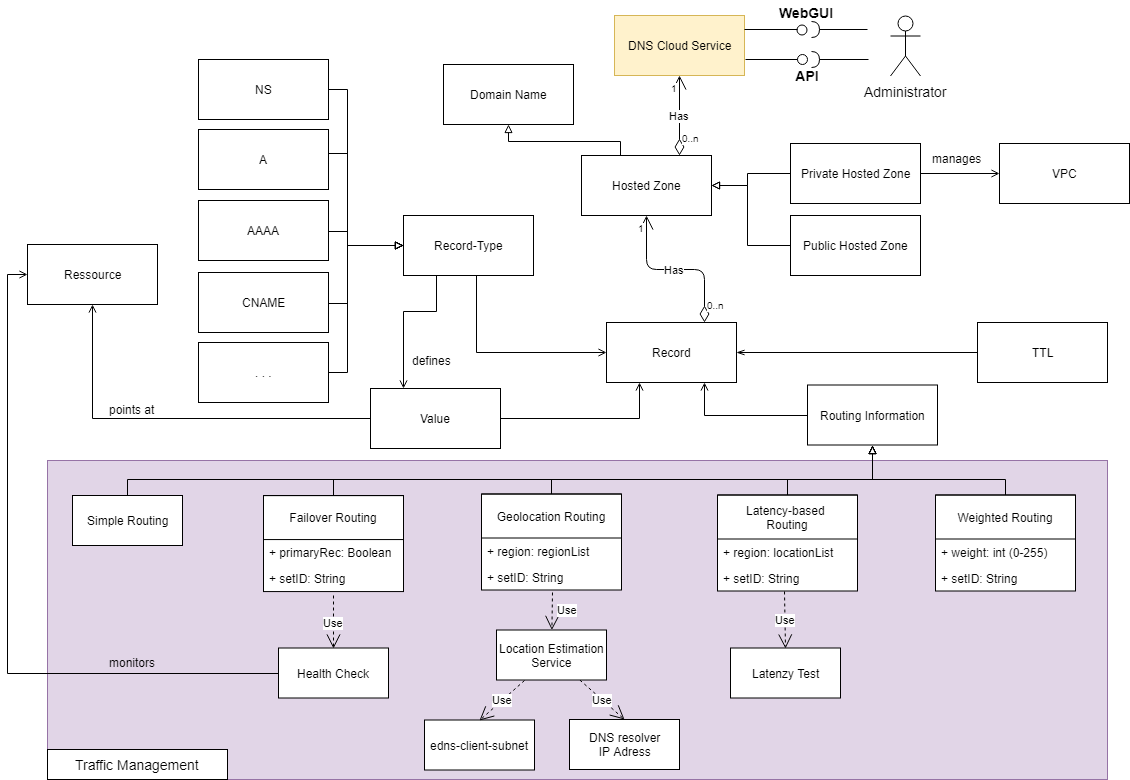
\includegraphics[width=\textwidth]{images/cc_modelxml.png}
    \caption{Modell zur Beschreibung von DNS-Cloud-Services}
    \label{fig:ccmodel}
\end{sidewaysfigure*}

\subsection{Erstellung des Modells}
Zunächst war es notwendig sich auf dem Markt umzusehen um geeignete Anbieter von Cloud-Dienstleistern zu identifizieren. Anschließend wurden Kriterien gewählt, anhand deren die Anzahl der Alternativen eingeschränkt wurde. Daraufhin war es notwendig einen Einblick in die ausgewählten DNS-Services zu erlangen, die Funktionsweise dieser nachzuvollziehen und zu studieren. 

\subsection{Auswahl der Cloud-DNS-Serviceprovider}
Der Markt an DNS-Serviceprovidern ist enorm groß. Das meist genutzte Benchmark zum Vergleich von DNS-Services ist offensichtlich die benötigte Zeit zur direkten Auflösung einer DNS-Querry. Laut des DNS-Benchmarking Service \textit{DNSPerf} sind die Abweichungen der ersten 30 Plätze hier bei gerade einmal 30ms. Auch die Verfügbarkeit der einzelnen DNS-Server beläuft sich in den letzten 6 Monaten bei den ersten 30 Plätzen ebenfalls durchgängig bei 100\%. Bei anderen Benchmarking-Services waren ebenfalls ähnliche Werte zu verzeichnen.

Da eine Abweichung von 30ms bei der Bearbeitung einer DNS-Querry bei den meisten Endnutzern im täglichen Gebrauch kaum ins Gewicht fallen dürfte, wurde dies im weiteren Verlauf nicht weiter berücksichtigt. Auch eine Verfügbarkeit von 100\% scheint dem allgemeinen Standard zu entsprechen.